\documentclass[serif, aspectratio=169]{beamer}
\usepackage[T1]{fontenc} 
\usepackage{fourier}
\usepackage{hyperref}
\usepackage{latexsym,amsmath,xcolor,multicol,booktabs,calligra}
\usepackage{booktabs} % For better table formatting
\usepackage{graphicx,pstricks,listings,stackengine}
\usepackage{listings}
\usepackage{array} 
\usepackage{colortbl}

\author{Dr.Hajialiasgari}
\title{Machine Learning}
\institute{
    Tehran University \\
    Of\\
    Medical Science
}
\date{\small \today}
\usepackage{UoWstyle}

% Define custom colors and styles for listings
\definecolor{deepblue}{rgb}{0,0,0.5}
\definecolor{deepred}{RGB}{153,0,0}
\definecolor{deepgreen}{rgb}{0,0.5,0}
\definecolor{halfgray}{gray}{0.55}

\lstset{
    basicstyle=\ttfamily\small,
    keywordstyle=\bfseries\color{deepblue},
    emphstyle=\ttfamily\color{deepred},
    stringstyle=\color{deepgreen},
    numbers=left,
    numberstyle=\small\color{halfgray},
    rulesepcolor=\color{red!20!green!20!blue!20},
    frame=shadowbox,
}

\begin{document}

\begin{frame}
    \titlepage
    \vspace*{-0.6cm}
    \begin{figure}[htpb]
        \begin{center}
            \includegraphics[keepaspectratio, scale=0.05]{Tumsl-logo.png}
        \end{center}
    \end{figure}
\end{frame}

\begin{frame}    
\tableofcontents[sectionstyle=show, subsectionstyle=show/shaded/hide, subsubsectionstyle=show/shaded/hide]
\end{frame}

\section{Regression}
\begin{frame}{Introduction To Regression}
     \begin{itemize}
         \item The term "Regression" was coined by Francis Galton in the 19th century to describe a biological phenomenon. The phenomenon observed was that the height of descendants of tall ancestors tends to regress downward. For Galton, regression had only this biological meaning, but his work was later extended to a broader statistical context by Udny Yule and Karl Pearson.
     \end{itemize}
    
\end{frame}


\section{What is a Model?}
\begin{frame}
    \begin{itemize}
        \item A model in machine learning works like a function: it takes input data, processes it based on learned patterns, and produces an output, such as predictions or classifications.
    \end{itemize}
\end{frame}


\section{Solution Components - Learning Model}

\begin{frame}{Hypothesis Set}
    \textbf{Definition:} The set of all possible models or functions \( h(x, \theta) \) that the learning algorithm can choose from.

    \vspace{0.3cm}
    \textbf{Mathematics:}
    \[
    h(x, \theta) = f(x_1, x_2, \dots, x_n; \theta_1, \theta_2, \dots, \theta_m)
    \]
    \begin{itemize}
        \item \( x \): Input features.
        \item \( \theta \): Model parameters (e.g., weights, biases).
    \end{itemize}

    \vspace{0.3cm}
    \textbf{Example (Linear Regression):}
    \[
    h(x, \theta) = \theta_0 + \theta_1 x_1 + \theta_2 x_2
    \]
\end{frame}


\begin{frame}{Learning Model Overview}
	\textbf{Hypothesis Set:}  
	A collection of functions \( h(x, \theta) \) that maps input \( x \) to output \( y \), parameterized by \( \theta \).
	
	\[
	h(x, \theta) = f(x_1, x_2, \dots, x_n; \theta_1, \theta_2, \dots, \theta_m)
	\]
\end{frame}

\begin{frame}{Linear Hypothesis Space}
    \begin{itemize}
        \item \textbf{Simplest form:} Linear combination of input features.
        \[
        h_w(x) = w_0 + \sum_{i=1}^{D} w_i x_i
        \]

        \item \textbf{Linear Hypothesis Examples:}
        \begin{itemize}
            \item \textbf{Single Variable:} 
            \[
            h_w(x) = w_0 + w_1 x
            \]
            \item \textbf{Multivariate:} 
            \[
            h_w(x) = w_0 + w_1 x_1 + w_2 x_2 + \dots + w_D x_D
            \]
        \end{itemize}
    \end{itemize}
\end{frame}

\begin{frame}{Understanding Cost Functions}
    \begin{itemize}
        \item In the hypothesis space, we select a function \( h(x; w) \) to approximate the true relationship between input \( x \) and output \( y \).
        \item The objective is to minimize the difference between predicted values \( h(x) \) and actual values \( y \).
        \item This difference is quantified using \textbf{cost functions}, which guide us in choosing the optimal hypothesis.
    \end{itemize}
\end{frame}

\begin{frame}{What is a Cost Function?}
    \begin{itemize}
        \item A cost function measures how well the hypothesis 
         $h(x; w)$ fits the training data.
    
        \item In regression problems, the most common error function is the \textbf{Squared Error (SE)}:
        \[
        SE = \left( y^{(i)} - h(x^{(i)}; w) \right)^2
        \]
    
        \item The cost function should measure all predictions. Thus, a possible choice is the \textbf{Sum of Squared Errors (SSE)}:
        \[
        J(w) = \sum_{i=1}^{N} \left( y^{(i)} - h(x^{(i)}; w) \right)^2
        \]

        \item \textbf{Objective:} Minimize the cost function to find the best parameters $w$.
\end{itemize}
\end{frame}

\begin{frame}{SSE: Sum of Squared Errors}
    \begin{itemize}
        \item \textbf{SSE} is widely used due to its simplicity and differentiability.
        \item Intuitively, it represents the squared distance between predicted and true values.
        \item Penalizes larger errors more severely than smaller ones (due to the square).
        \item For linear regression, it can be written as:
        \[
        SSE = \sum_{i=1}^{N} \left( y^{(i)} - \mathbf{w}^T \mathbf{x}^{(i)} \right)^2
        \]
    \end{itemize}    
\end{frame}

\begin{frame}{How to measure the error}

    \begin{figure}[h]
        \centering
        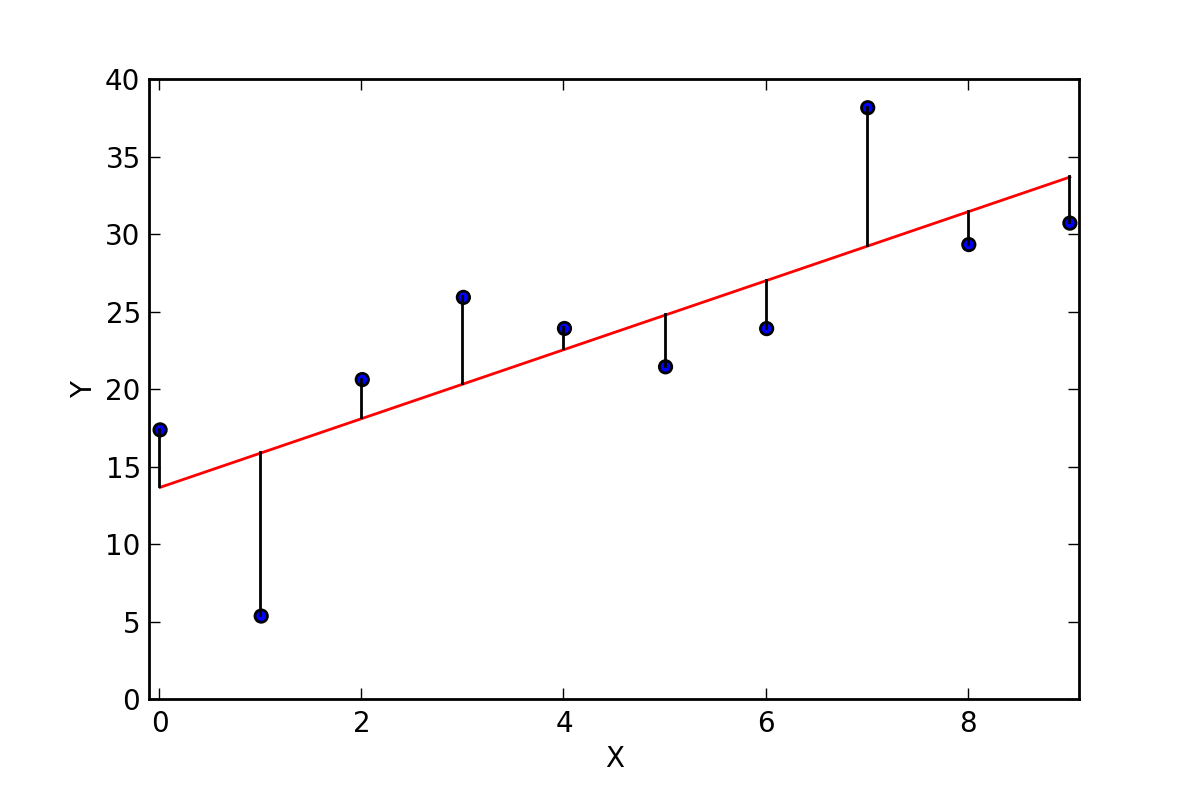
\includegraphics[width=0.5\textwidth]{MAE.png} 
    \end{figure}
    \[
    J(w) = \sum_{i=1}^{n} \left( y^{(i)} - h_w(x^{(i)}) \right)^2 = \sum_{i=1}^{n} \left( y^{(i)} - w_0 - w_1 x^{(i)} \right)^2
    \]
\end{frame}

\begin{frame}{Cost Function Optimization}
    \item The goal of linear regression is to minimize the sum of squared errors (SSE) between the predicted values and the actual values.
    
    \begin{equation}
    J(w) = \sum_{i=1}^{n} \left( y^{(i)} - w_0 - w_1 x^{(i)} \right)^2
    \end{equation}
\end{frame}

\begin{frame}{Condition For Optimal Value}
    \item To find the optimal values of $w_0$ and $w_1$, we need to solve the following partial derivatives and set them to zero:
    \begin{equation}
    \frac{\partial J(w)}{\partial w_0} = 0
    \end{equation}

    \begin{equation}
    \frac{\partial J(w)}{\partial w_1} = 0
    \end{equation}
\end{frame}

\begin{frame}{Optimization}
    \begin{figure}[h]
        \centering
        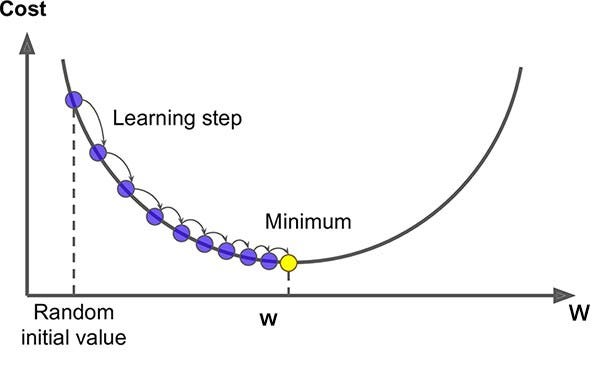
\includegraphics[width=0.5\textwidth]{OptReg.jpg} 
    \end{figure}
\end{frame}

\section{Linear Regression}


\begin{frame}
    \begin{center}
        {\Huge\ \color{red}For more information and code check the related notebook}
    \end{center}
\end{frame}


\begin{frame}
    \begin{center}
        {\Huge\ End of Regression}
    \end{center}
\end{frame}

\end{document}

